\section{Monday 11/04/2024}
\subsection{Optimization Algorithms for Unconstrained Problems 3}
\subsubsection{Meta-Heuristics}
There are heuristic optimization algorithms that try to exploit some intuitive understanding of the original problem and use that to find the best solution instead of some problem-agnostic algorithm like gradient descent. Genetic algorithms are algorithms that create different generations of solutions with characteristics and a "fitness" score. At each iteration, the probability of an algorithm surviving is defined by its fitness score and then a new generation is created from the solutions that survived. At each generation, there is a mutation process that can introduce new characteristics into the solutions.
\subsection{Optimization Algorithms for Constrained Problems}
A constrained optimization problem can be transformed into an unconstrained problem by introducing a cost to each constraint in the objective function.
\begin{equation}
  \begin{aligned}
    \text{minimize } f(x) \\
    \text{subject to } g(x) \leq 0 \\
    h(x) = 0
  \end{aligned}
\end{equation}
Can be turned into
\begin{equation}
  \text{minimize } f(x) + \lambda g(x) + \nu h(x)
\end{equation}

\subsubsection{Projection-based method}
Mirror descent is an optimization method that allows us to alter the unconstrained case of gradient descent and change it into the constrained case. We introduce the domain and restrict it to a convex set $\Omega \subseteq \mathbb{R}^d$

\section{Wednesday 11/06/2024}
\subsection{Projection-based Methods}
Projection-based methods work well with gradient methods, also known as first-order methods. 
\subsubsection{Mirror Descent}
For some convex set $\Omega \subseteq \mathbb{R}^d$, we can change the unconstrained gradient descent from 
\begin{equation}
  \min_{x \in \mathbb{R}^d } f(\textbf{x}^{k-1}) + \langle \nabla f(\textbf{x}^{k-1}), \textbf{x} - \textbf{x}^{k-1}  \rangle + \frac{1}{2 \alpha^{k-1}} \| \textbf{x} - \textbf{x}^{k-1} \|_2^2
\end{equation}
to 
\begin{equation}
  \min_{x \in \Omega } f(\textbf{x}^{k-1}) + \langle \nabla f(\textbf{x}^{k-1}), \textbf{x} - \textbf{x}^{k-1}  \rangle + \frac{1}{2 \alpha^{k-1}} \| \textbf{x} - \textbf{x}^{k-1} \|_2^2
\end{equation}
This works because we are taking the feasible region that would otherwise be defined by the constraints $g(x),h(x)$ and we bring the intersection of all constraints into the minimization problem. Frequently, these convex sets fall into the general sets below:
\begin{itemize}
  \item $\Omega = \{ x | x \geq 0 \}$
  \item $\Omega = \{ x | a \leq x \leq b \}$
  \item $\Omega = \{ x | \| x \| \leq R \}$
\end{itemize}

The previous equation is also equivalent to euclidean projection.
\begin{equation}
  \min_{x \in \Omega} \frac{1}{2} \| \textbf{x}^{k-1} - \alpha^{k-1} \nabla f(\textbf{x}^{k-1}) - \textbf{x}\|_2^2
\end{equation}
Here, we can bring back the definition that $\textbf{x}^k = \textbf{x}^{k-1} - \alpha^{k-1} \nabla f(\textbf{x}^{k-1})$. This means that the above equation can be interpreted as us finding the $\textbf{x}$ that is closest to our previous (potentially infeasible) guess of $\textbf{x}^k$. In other words, we are letting gradient descent pick infeasible or feasible solutions, and then we are finding the projection of the infeasible solutions onto the feasible region.
\subsubsection{Non-negative set}
If we define $\Omega = \{ x | x \geq 0 \}$ we can write the gradient descent as 
\begin{equation}
  \min_{x \geq 0 } \| \textbf{y}^k - \textbf{x}\|_2^2
\end{equation}
where the optimal solution is
\begin{equation}
  x_i = 
  \begin{cases}
    y_i^k & y_i^k \geq 0 \\
    0 & o.w.
  \end{cases}
\end{equation}
In this special case where the domain is restricted to $\Omega = \{ x | x \geq 0 \}$, this also applies for any norm in this specific set.

\subsubsection{Upper/Lower bounds}
Now we define the convex set that restricts the gradient descent domain as $\Omega = \{ x | a \leq x \leq b \}$
\begin{equation}
  \min_{a \leq x \leq b } \| \textbf{y}^k - \textbf{x}\|_2^2
\end{equation}
where the optimal solution is
\begin{equation}
  x_i = 
  \begin{cases}
    y_i^k & y_i^k \in [a_i,b_i] \\
    b_i & y_i^k > b_i \\
    a_i & y_i^K < a_i
  \end{cases}
\end{equation}
This is also a rather trivial solution. 
\subsubsection{Euclidean ball}
Now we define the convex set as $\Omega = \{ x | \| x \|_2 \leq R \}$. This is a euclidean ball with radius $R$.

\begin{equation}
  \min_{\| x \|_2 \leq R} \| \textbf{y}^k - \textbf{x}\|_2^2
\end{equation}

In this case, if the fixed point $y^k$ is outside of the feasible region, the point on the edge of the feasible region will have a tangent with a normal that runs through the point $y^k$.
\begin{figure}[htbp]
  \centerline{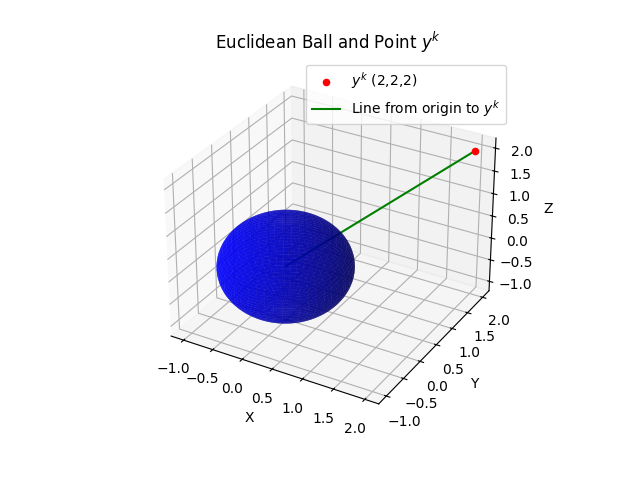
\includegraphics[width=0.75\textwidth]{images/euclidean_ball.png}}
  \caption{Euclidean ball with the infeasible point $y^k$}
  \label{fig:euclidean_ball}
\end{figure}

The optimal solution here is
